%!TEX program = xelatex
\documentclass{article}
\usepackage{fancyhdr}
\usepackage{extramarks}
\usepackage{amsmath}
\usepackage{amsthm}
\usepackage{amsfonts}
\usepackage{tikz}
\usepackage[plain]{algorithm}
\usepackage{algpseudocode}
\usepackage{enumerate}
\usepackage{graphicx}
\usepackage{pythonhighlight}
\usepackage{amssymb}
\usepackage{ctex}
\usepackage{listings}
\usepackage{subfigure}

\usetikzlibrary{automata,positioning}

%
% Basic Document Settings
%  

\topmargin=-0.45in
\evensidemargin=0in
\oddsidemargin=0in
\textwidth=6.5in
\textheight=9.0in
\headsep=0.25in

\linespread{1.1}

\pagestyle{fancy}
\lhead{\hmwkAuthorName}
\chead{\hmwkClass\ (\hmwkClassInstructor): \hmwkTitle}
\rhead{\firstxmark}
\lfoot{\lastxmark}
\cfoot{\thepage}

\renewcommand\headrulewidth{0.4pt}
\renewcommand\footrulewidth{0.4pt}

\setlength\parindent{0pt}

%
% Create Problem Sections
%

\newcommand{\enterProblemHeader}[1]{
    \nobreak\extramarks{}{Problem \arabic{#1} continued on next page\ldots}\nobreak{}
    \nobreak\extramarks{Problem \arabic{#1} (continued)}{Problem \arabic{#1} continued on next page\ldots}\nobreak{}
}

\newcommand{\exitProblemHeader}[1]{
    \nobreak\extramarks{Problem \arabic{#1} (continued)}{Problem \arabic{#1} continued on next page\ldots}\nobreak{}
    \stepcounter{#1}
    \nobreak\extramarks{Problem \arabic{#1}}{}\nobreak{}
}

\setcounter{secnumdepth}{0}
\newcounter{partCounter}
\newcounter{homeworkProblemCounter}
\setcounter{homeworkProblemCounter}{1}
\nobreak\extramarks{Problem \arabic{homeworkProblemCounter}}{}\nobreak{}

%
% Homework Problem Environment
%
% This environment takes an optional argument. When given, it will adjust the
% problem counter. This is useful for when the problems given for your
% assignment aren't sequential. See the last 3 problems of this template for an
% example.
%
\newenvironment{homeworkProblem}[1][-1]{
    \ifnum#1>0
        \setcounter{homeworkProblemCounter}{#1}
    \fi
    \section{Problem \arabic{homeworkProblemCounter}}
    \setcounter{partCounter}{1}
    \enterProblemHeader{homeworkProblemCounter}
}{
    \exitProblemHeader{homeworkProblemCounter}
}

%
% Homework Details
%   - Title
%   - Due date
%   - Class
%   - Section/Time
%   - Instructor
%   - Author
%

\newcommand{\hmwkTitle}{FinalProject}
\newcommand{\hmwkDueDate}{July 1st, 2020}
\newcommand{\hmwkClass}{Reinforcement Learning}
\newcommand{\hmwkClassInstructor}{Professor Ziyu Shao}
\newcommand{\hmwkAuthorName}{Tianyuan Wu}
\newcommand{\hmwkAuthorID}{63305667}

%
% Title Page
%

\title{
    \vspace{2in}
    \textmd{\textbf{\hmwkClass:\ \hmwkTitle}}\\
    \normalsize\vspace{0.1in}\small{Due\ on\ \hmwkDueDate\ at 11:59pm}\\
    \vspace{0.1in}\large{\textit{\hmwkClassInstructor}}
    \vspace{3in}
}

\author{\textbf{\hmwkAuthorName}\\ \hmwkAuthorID}
\date{}

\renewcommand{\part}[1]{\textbf{\large Part \Alph{partCounter}}\stepcounter{partCounter}\\}

%
% Various Helper Commands
%

% Useful for algorithms
\newcommand{\alg}[1]{\textsc{\bfseries \footnotesize #1}}

% For derivatives
\newcommand{\deriv}[1]{\frac{\mathrm{d}}{\mathrm{d}x} (#1)}

% For partial derivatives
\newcommand{\pderiv}[2]{\frac{\partial}{\partial #1} (#2)}

% Integral dx
\newcommand{\dx}{\mathrm{d}x}

% Alias for the Solution section header
\newcommand{\solution}{\textbf{\large Solution}}

% Probability commands: Expectation, Variance, Covariance, Bias
\newcommand{\E}{\mathrm{E}}
\newcommand{\Var}{\mathrm{Var}}
\newcommand{\Cov}{\mathrm{Cov}}
\newcommand{\Bias}{\mathrm{Bias}}

\begin{document}

\maketitle

\pagebreak

\begin{homeworkProblem}
    \textbf{Solution}\\
    在此课程中,我学习到了许多与强化学习相关的算法,并加深了对基础数学知识的了解。总体来说,我认为此课程基本
    满足了我对强化学习课程的期望,但还有些部分还有改进的空间。比如,我希望了解更多与深度强化学习相关的内容,
    比如DQN、PPO等最近流行的算法。此外,我认为作业可以少一些重复性的复现类的内容,多一些和前沿内容接轨的内容,
    或数学推导类的内容。
\end{homeworkProblem}

\begin{homeworkProblem}
    \textbf{Solution}\\
    \textbf{The code implementation of the problem is in ``problem2.ipynb''}
    \begin{enumerate}
    \item[a) ] MCMC method\\
        First, we analysis the problem theoretically. The maximum cut problem is quite similar like the independent set problem, and we can solve 
        it by similar ways. we have 2 sets $A$ and $B$, the size of the cut $(A,B)$ is the number of edges that crosses $A$ and $B$.
        The basic idea is, use a binary sequence to represent the choice of . $s[i] = 0$ means choose vertex 
        $i$ in $A$, and $s[i] = 1$ means choose it in $B$. Then, construct a irreducible Markov Chain, each sate $X_i$ represent a binary sequence, and in each iteration, 
        we filp a bit randomly, and go to the new state. \\
        Then, the stationary distribution $\pi$ of this chain is an uniform distribution. Then, we can modify the chain to make 
        it concentrate on states with larger size of the cut (i.e. larger number of crossing edges from A to B), by MH method. That is, filp a coin with 
        $p_H = e^{\beta(V_{new} - V_{curr})}$, where $V_{s_i} = \#\ of\ 1s\ in\ s_i$. Then if the coin landing head, accept the proposal, otherwise 
        reject the proposal.\\
        That idea can be described in details as:
        \begin{enumerate}
        \item [1)] Label all vertices by a number $0, 1, \ldots, n$
        \item [2)] Init the sequence to $s_i =(000\ldots 0)_n$, $0$ means the vertex is in the set $A$, and $1$ means it's in set $B$.
        \item [3)] Generate a random number $k = [0, n-1]$, and filp the bit at index $k$, to get the new state $s_{new}$.
        \item [4)] Let $V_{s_i} = \text{cutSize}(A, B)$, filp a coin with probability of landing head $p = e^{\beta(V_{new} - V_{curr})}$
        \item [5)] If the coin landing head, accept the proposal, otherwise reject the proposal.
        \item [6)] Jump to step (3)
        \end{enumerate}
        We do simulation $10^4$ steps, and we can observe the maximum cut size is 24.
        we run it several times, and some of the simulation results are shown below: 
        \begin{lstlisting}
        ============== MCMC method ===============
        The maximum cut is:
        S1 = {1,3,4,7,9,11,14,15,18,20},
        S2 = {2,5,6,8,10,12,13,16,17,19},
        with reward = 24
        \end{lstlisting}
        The result is the same as the optimal solution (size=24).
        \newline
    \item [b)] Cross-entropy method\\
        The basic idea is quite simple. Same as the MCMC method, we still use a binary sequence to represent the 
        selection of vertices. First, we generate $N$ episodes. In each episode, for each vertex, we decide it 
        in $A$ or $B$ with equal probability (i.e. for each sequence $s$, $\Pr[s[i] = 0] = \Pr[s[i] = 1] = 0.5$). 
        Then, calculate the cut size of each episode, and select $k = N/2$  elite samples in these $N$ samples. 
        Then, update the probability of sampling each vertex by the CEM equation:
        $$\hat{p}_{i,j} = \frac{\sum_{j=0}^{N}I\{S(X_i) \ge \hat{\gamma}_t\} I\{X_{i,j}=1\}}{\sum_{j=0}^{N}I\{S(X_i) \ge \hat{\gamma}_t\}}$$
        For example, if we choose 4 elite samples, 3 of them choosed vertex $i$ in set $A$, and only 1 of them choosed 
        vertex $i$ in $B$, then we will update 
        $$\Pr[\text{choose vertex i in A}] = \frac{3}{4}$$
        \begin{enumerate}
            \item [1)] Label all vertices by a number $0, 1, \ldots, n$
            \item [2)] Init the sequence to $s_i =(000\ldots 0)_n$, $0$ means the vertex is in the set $A$, and $1$ means it's in set $B$.
            \item [3)] Init the probability distribution $\textbf{p} = [p_1, p_2, \ldots, p_n]$
            \item [4)] Generate $N$ samples from the probability distribution $\textbf{p}$
            \item [5)] Select $k$ elite samples from $N$ samples
            \item [6)] Use these elite samples to update $\textbf{p}$
            \item [7)] Goto (4)
        \end{enumerate}        
        We do simulation $100$ steps, which each step choose $500$ samples, and we can observe the maximum cut size is 24.
        we run it several times, and some of the simulation results are shown below: 
        \begin{lstlisting}
        ==========Cross Entropy method==========
        The maximum cut is:
        S1 = {1,3,4,7,10,11,14,17,18,20},
        S2 = {2,5,6,8,9,12,13,15,16,19},
        with reward = 24
        \end{lstlisting}
        The result is the same as the optimal solution (size=24).
        \newline
    \item [c)] MCTS method\\
        Similarly, we still use a binary sequence to represent the the selection of vertices.
         In initial case (root of the tree), all nodes are in the same set $A$
        (the sequence is $(000...00)$). And each action is, ``filp'' a bit in the sequence (choose 
        some vertex and put it in the other set), the value of a node is $V_i = \text{cutSize}(A, B)$. 
        Then we follows the MCTS algorithm with UCB method (i.e. when choose a children, we follows 
        the following equation):
        $$\text{BestChildren of v} = argmax_{v' \in children(v)}\frac{Q(v')}{N(v')} + c\sqrt{\frac{2\ln N(v)}{N(v')}}$$
        where $Q(v)$ is the value of the node, $N(v)$ is the visit count of $v$.
        We do simulation $5000$ steps, and we can observe the maximum cut size is 24.
        we run it several times, and some of the simulation results are shown below:  
        \begin{lstlisting}
        ============== MCTS method ===============
        The maximum cut is:
        S1 = {1,3,6,8,9,10,14,17,18,20},
        S2 = {2,4,5,7,11,12,13,15,16,19},
        with reward = 24
        \end{lstlisting}
        The result is the same as the optimal solution (size=24).
        \newline
    \item [d)] Discussion \& Comparison\\
        In this problem, MCMC method without MH method will get a uniform distribution of all cuts, which 
        may hard to find the optimal one. Suppose the graph is large, and the number of max cut is small (e.g. only one 
        max cut), MCMC method need to run a large number of steps until find the max cut. If we use MH 
        method in MCMC, then we have higher probability to visit the larger cuts, which may mitigate this 
        problem. The advantage is, in each iteration, MCMC method is very fast. Unlike CEM or MCTS, 
        in this problem, MCMC method only need to filp a bit and go to the next state in each iteration, 
        which is faster than other methods.\\
        CEM method is based on importance sampling. 
        When we use CEM method, we need to consider the equilibrium between number of samples in each iteration ($N$)
        and the number of iterations.  If $N$ is small, we may need large number of iterations until converge, 
        but if $N$ is large, the calculation time in each iteration will be longer. In conclusion, CEM is 
        a importance sampling based method, which is better than uniform sampling MCMC method. But we need a 
        suitable $N$ and proportion $p$ of elite samples to make it converge faster.\\
        MCTS is based on tree traversal. In each iteration, we go down the tree from root to the leaf. 
        Each time we will choose the children with best value calculated by UCB algorithm. If we visit 
        a node that we never visited, we will do a roll-out, otherwise we will expand it. This method is 
        suitable for problems with large number of state spaces, and will get the optimal solution with high probability
        if we iterates enough time, which is much better than MCMC, but each iteration of MCTS is much slower than MCMC.        
    \end{enumerate}
\end{homeworkProblem}

\begin{homeworkProblem}
    \textbf{Solution}\\
    \begin{enumerate}
        \item [1)] \textbf{Human-level control through deep reinforcement learning, by Mnih et al, Nature, 2015}\\
            Main contributions: This article presents the Deep Q network, which is now widely used 
            various subjets of deep reinforcement learning. This is a single algorithm that would be used 
            in a wide range of challenging tasks. The main idea of Deep Q network is 
            to combine the deep neural networks and the reinforcement learning algorithms. That is, use the 
            deep neural networks to represent the Q value (state-action value) of some state $Q^*(s, a)$.  
            We know that in traditional reinforcement learning algorithms, the target is to maximize the total reward, which is a quite 
            difficult nonlinear problem:
            $$Q^*(s, a) = \max_{\pi} \mathbb{E}[r_t + \gamma r_{t+1}+ \gamma^2 r_{t+2} + \ldots | s_t=s, a_t=a, \pi]$$
            In this article, the author use deep convolutional networks to approximate $Q^*(s, a)$. That is, use $Q(s,a;\theta_i)$ 
            to represent the Q value at $(s, a)$, and $\theta _i$ is the parameters of the DQN at iteration $i$. Then, 
            use the observed samples to calculate the loss and update the network, the loss is shown as: 
            $$L_i(\theta_i) = \mathbb{E}_{(s, r, a, s')}[(r + \gamma \max_{a'} Q(s,a;\theta_i^-) - Q(s,a;\theta_i))^2]$$
            Also, the author tests the performance of DQN on many classical games, and more than a half of them 
            are at or above human level.\\
            What is surprising is, the input is only the pixels which is the same as what's human seen, and the CNN can 
            almost do the prediction as well as what's human did. That shows that CNNs can not only be used on fileds such 
            as computer vision or image processing, but can also be used in more general problems.\\
            What's difficult is, DQN is only suitable when the state space is discrete, and the performance of DQN 
            is not stable (we can observe that the variance of avg. scores shown in Fig. 2(a) and 2(b) is quite high). \\
            In my opinion, the experiments is convincing. Because the author tested the performance on various of 
            games, most but not all of them are quite good. Also, the author offers the code, and I actually run part of them on 
            my computer, the results are similar as which were shown in the paper.\\
            Related works: The DQN is applied in multi-agent game StarCraft II:
            ``Grandmaster level in StarCraft II using multi-agent reinforcement learning, Oriol Vinyals, Nature 2019''.

        \item [2)] \textbf{Mastering the game of Go with deep neural networks and tree search, by Silver et al, Nature 2016}\\
            Main contribution: This article presents the AlphaGo, a new approach to computer Go that uses value networks
            to evaluate board positions and policy networks to select moves. The main difference between this algorithm 
            and other algorithms is, AlphaGo not only learn from human expert games, but also learn from self-plays. 
            The authors used MCTS method with value network and policy network to evaluate the optimal action. They first 
            use supervised learning (SL) method to train policy 13-layered network $p_\pi$ directly from human expert games, 
            which uses stochastic gradient descent to maximize the likelihood of human move state-action pair $(s,a)$. 
            Then, they trained an reinfoecement learning(RL) policy network $p_\rho$, to improve the performance of 
            SL policy network by optimizing the final outcomes of self-play. 
            Finally, a value network $v_\theta$ is trained to predict the winner of the game. 
            In the MCTS search process, each edge of the tree represents a state action pair $(s,a)$, and for each time, 
            choose action by:
            $$a_t = arg\max_{a}(Q(s_t, a) + u(s_t, a))$$
            where $u(s_t, a) \propto \frac{P(s,a)}{1+N(s,a)}$ that is proportional to the prior probability but decays with repeated visits to encourage exploration.
            Also, the author tested the performance of AlphaGo, it achieved $99.8\%$ winning rate of 
            other Go programs, and reached the expert level among human.\\
            What is surprising is, they first trained a SL policy network by human experiments, then use RL 
            methods to improve this network which can significantly reduce the training time and get better 
            performance. This method can not only let the agent learn from the self-play experiments, but also 
            bring human knowledges to the agent. \\
            The difficultity is, this method highly depends on the human experts' game knowledge, and the training and evaluation 
            speed may need a large amount of computing resources.\\
            I think the experiments is convincing, for the article provides enough information to prove 
            the conclusion, and the performance of AlphaGo has already been proved by winning many Go competitions between AI and 
            human experts.\\
            Related works: This is an article about computational chemistry, they uses chemists' knowledge and RL methods 
            to predict and invent chemical reactions: ``Modelling Chemical Reasoning to Predict and Invent Reactions, 
            Marwin H. S. Segler and Mark P. Waller, Chem. Eur. J. 2017, 23, 6118 – 6128''

        \item [3)] \textbf{Mastering the game of Go without human knowledge, by Silver et al, Nature 2017}\\
            Main contributions: This article presentes the AlphaGo Zero, a Go program without human knowledge. 
            The neural networks of AlphaGo Zero is trained only from games of self-play by a reinforcement learning 
            algorithm. For each board state $s$,  the neural network $f_\theta$ is able to give a probability vector $p$,
            and a value $v$. $p_a = \Pr[a|s]$ is the probability of taking action $a$ at state $s$. Same as AlphaGo, 
            AlphaGo Zero still used MCTS method. The MCTS guided by the policy network $f_\theta(s)$ to get the probabilities of 
            policy $\pi$ (Use MCTS as a powerful policy improvement operator). Also, use self-play with search as a 
            policy evaluation operator. That is, do the following procedure repeatedly, \\
            (1). Update the parameters of network to make $(p, v) = f_\theta(s)$ more close to the winner's policy and 
            the improved search probability\\
            (2). Use the new parameters $\theta^-$ to make the search stronger.\\
            The purpose of the neural network is to minimize the difference (error) between 
            what it predicted ($v$) and the winner's history $z$, 
            and to maximize the similarity between the move probabilities $p$ given by the network and the search
            probabilities $\pi$. So, the loss is:
            $$L = (z-v)^2 -\pi^T \log p + c||\theta||^2$$
            Where $c||\theta||^2$ is the L2 weight regularization to prevent overfitting.\\
            Then, the author tested the performance of AlphaGo Zero, and when the training time is enough, 
            the performance finally be better than AlphaGo Lee and AlphaGo Master. \\
            What's surprising is, the MCTS and neural networks can be combined together, and ``help'' 
            each other to improve the performance. The evaluation results of AlphaGo Zero is better than 
            AlphaGo is also a surprising result. That means the human experts' game knowledge may not be always 
            correct, and AI may learning something new by self-play. What's difficult is, the training process 
            without human knowledge will take longer time, and need more computing resources.\\
            I think the experiments is convincing, for vaild evidents are given to prove the result of training process. 
            Also, AlphaGo Zero is also proved by winning many worldwide Go competitions. \\
            Related worls: This is also an article about computational chemistry, they use MCTS and similar training process, and it aims to 
            help chemists with organic syntheses: ``Planning chemical syntheses with deep neural networks and symbolic AI, 
            Segler, Marwin H. S,Preuss, Mike,Waller, Mark P, Nature 2018''

        \item [4)] \textbf{A general reinforcement learning algorithm that masters chess, shogi, and Go through self-play, by Silver et al, Science 2018}\\
            Main contributions: This article presents AlphaZero, a general RL algorithm for chess, shogi, and Go.
            In earlier programs for chess-like games, a large amount of domain-specific human knowledge is needed in order 
            to make the optimal decision. But AlphaZero used a self-play based RL algorithm, which means it can 
            ``learn'' the game without human knowledge. Instead of using handcrafted evaluation functions and weights, 
            AlphaZero uses a deep neural network $f_\theta(s)$ to give the values $v$ and probability vector $p$ indicates 
            the probabilities of different moves. 
            $$(\textbf{p}, v) = f_{\theta}, \text{where } \textbf{p}=\Pr[a|s]$$  
            Same as AlphaGo Zero mentioned above, AlphaZero also uses a general MCTS method. In each iteration, 
            it searches from root until a leaf node with high probability to move to high-value nodes (exploitation), and low 
            probability to move to nodes with low visit count (exploration). Also the same as AlphaGo Zero, combine 
            neural network and MCTS together to ``help'' each other to improve the performance. So the loss function of 
            the neural network is also defined as $L = (z-v)^2 -\pi^T \log p + c||\theta||^2$. What different with 
            AlphaGo Zero is, AlphaZero simply maintains a single neural network that is updated continually rather 
            than waiting for an iteration to complete. AlphaZero is also tested on various chess-like games, and 
            has superhuman performances on chess, shogi, and Go. \\
            What's surprising is, almost all chess-like games can be solved by the MCTS + neural network moethod, 
            I've also seen that such approachs used in chemistry, computer vision and many different fileds. That means 
            the self-play based RL algorithm can work quite well when the state space is large and discrete. And the 
            difficulties is also very clear, these methods (without human knowledge) needs more time to train and 
            more computing resources to train and evaluate through it's more creative.  \\
            I also think that the results are convincing. For Go, chess and shogi are similar chess-like games, through 
            the rules are different. They all have large and discrete state space, the agent's action are also similar. 
            Due to AlphaGo Zero works quite well, this algorithm works also well on other similar games is convinced. \\
            Related works: This is an article about solving the Rubik's cube game with similar approach.
            ``Solving the Rubik's Cube Without Human Knowledge, McAleer, Stephen,Agostinelli, Forest,Shmakov, Alexander, 2018''
            
        \item [5)] \textbf{DeepStack: Expert-level artificial intelligence in heads-up no-limit poker, by Moravcik et al, Science, 2017}\\
            Main contributions: This article presents DeepStack, a new algorithm to solve problems with sequential imperfect information 
            (i.e. sequential problems/games with asymmetric information) such as poker. It uses the recursive reasoning of 
            counterfactual regret minimization (CFR) method to handle the asymmetric information, but it neither compute and store 
            the complete strategy prior, nor has need for explicit abstraction. Instead, it considers each particular situation as it arises 
            during play, but not in isolation. Also, the DeepStack solves an approximate Nash equilibrium in zero-sum games 
            (it computes and plays a low-exploitability strategy). The basic workflow of DeepStack is: It has a deep counterfactual value network
            trained by randomly generated poker situations. When it plays the poker game, for every public state it needs to act, 
            it resolves for its action by using a depth-limited lookahead where values of subtrees are computed by the network mentioned above.
            The author also tested the performance of DeepStack on HUNL games, it won 492mbb/g on average in as few as 3000 games, which 
            reaches the level of human experts.\\
            What's surprising is, the author use a depth limited search tree with and DNN to compute the value of subtrees instead of 
            simulate the whole game. It gets over the difficultity of the extremely large state space, and get a quite good 
            approximation. What's confusing is, I'm a little doubt the training process which uses randomly generated samples. 
            For the state space is large ($\sim 10^{160}$ in HUNL), maybe randomly generated samples cannot cover many special cases. \\
            I think this article is convincing in HUNL, for valid evidents are shown, and the performance is reasonable. 
            But on other poker games, I think it's just theoretically convinced, it's lack of evidence and experiments. \\
            Related works: This is an article about the optimtzation of DeepStack on Ludec Hold'em:
            ``Neural network optimtzation of algorithm DeepStack for playing in Leduc Hold'em, Yaroslav Yuriiovych DorogyiVasyl 
            Vasylovych Tsurkan,Vladyslav Yuriiovych Lisoviy, 2017
            ''
        \item [6)] \textbf{Safe and Nested Subgame Solving for Imperfect-Information Games, by Brown et al, NeurIPS, 2017}\\
            Main contributions: This article presents a new subgame solving technique on imperfect-information games which has 
            better performance than prior methods. In imperfect-information games, it is not possible to determine a subgame’s 
            optimal strategy using only knowledge of that subgame (i.e. cannot be solved in isolation), for the previous decisions 
            will make influence on current strategy. Although that cannot be solved only by subgames, this article 
            shows that it can be approximated by analyzing many disjoint subgames. Also, this article shows that by the 
            game progress down the game tree, the subgame solving can be repeated, which leads to far lower exploitation.
            Then, based on this subgame solving theory, the authors designed the first AI that can win top humans by 147 mbb/hand 
            in heads-up no-limit Texas hold’em poker, Libratus.\\
            What's surprising is, although the imperfect-imformation games cannot be solved directly by using subgames, 
            it can be well approximated by analyzing disjoint subgames. That is a creative and novel approach, especially for 
            the large space state games, even games with continues state space (need to be discritized). What's confusing is, 
            for I know little about the game theory and relative algorithms, I cannot realize part of theory such as 
            \texttt{reach margin}.\\
            Personally speaking, the experimental results is convincing, for the AI, Libratus, actually won the top level humans
            (Jason Lee, Dong Kim, Daniel McAulay and Jimmy Chou) in January 2017, Pittsburgh with a fairly judgement, which can 
            be seen in many reports.\\
            Related works: this article is the previous work of this paper published on NIPS 2017. It introduces the game 
            decomposition theory: 
            ``Solving Imperfect Information Games Using Decomposition, Neil Burch,Michael Johanson,Michael Bowling, AAAI'14''
    \end{enumerate}
\end{homeworkProblem}

\begin{homeworkProblem}
    \textbf{Solution}\\
    \textbf{The code implementation of this part is in the folder ``MyAlphaGomoku''}\\\\
    \textbf{Usage of my implementation:}
    \begin{itemize}
        \item This implementation needs dependencies \texttt{numpy}(for numeric calculations), 
        \texttt{pygame}(for GUI), \texttt{theano==0.8.2} and \texttt{lasagne==0.1.0} for running
        the original implementation (with deep neural network). 
        \item To start the game, use \texttt{python3 human\_play.py -forbidden} to run with forbidden rule, 
        \texttt{python3 human\_play.py -forbidden -usegui} to run with GUI and forbidden rule. 
        \texttt{python3 human\_play.py --help} to show usage information.
        \item You will first need to input if you want to go first, input \textbf{y} to go first, 
        \textbf{n} to go second.
        \item Then, you can choose your opponent, input \textbf{0} will play with another human, 
        \textbf{1} will play with the original AlphaZero (with neural network), \textbf{2} to play 
        with my RL agent which implemented without neural network.
        \item Player cannot put chess on forbidden locations, without GUI, forbidden locations are 
        shown as \textbf{F}, with GUI, forbidden locations are red `X'.
    \end{itemize}
    \begin{enumerate}
        \item[1)] Gomoku with Forbidden Rule\\
            In this problem, I implemented \textbf{almost all} forbidden rules.\\
            First, I implemented \textbf{Long forbiddens} (长连禁手 in Chinese).
            All four directions are supported:
            \begin{figure}[H]
                \centering
                \subfigure[long forbidden 1]{
                \begin{minipage}[t]{0.45\linewidth}
                \centering
                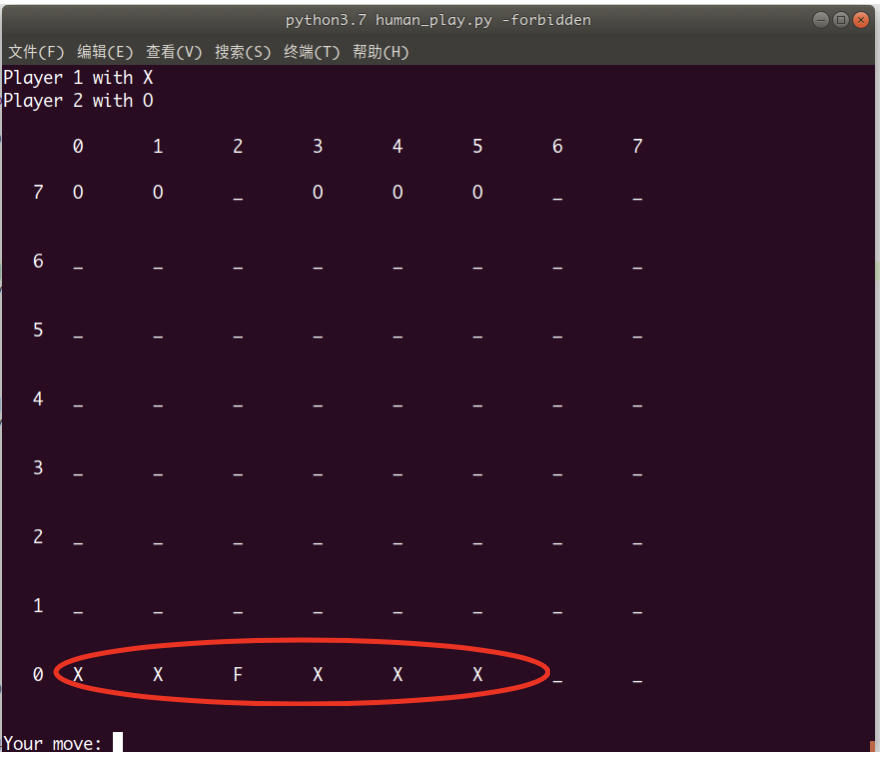
\includegraphics[width=0.85\linewidth]{./figs/l1.png}
                \end{minipage}%
                }%
                \subfigure[long forbidden 2]{
                \begin{minipage}[t]{0.45\linewidth}
                \centering
                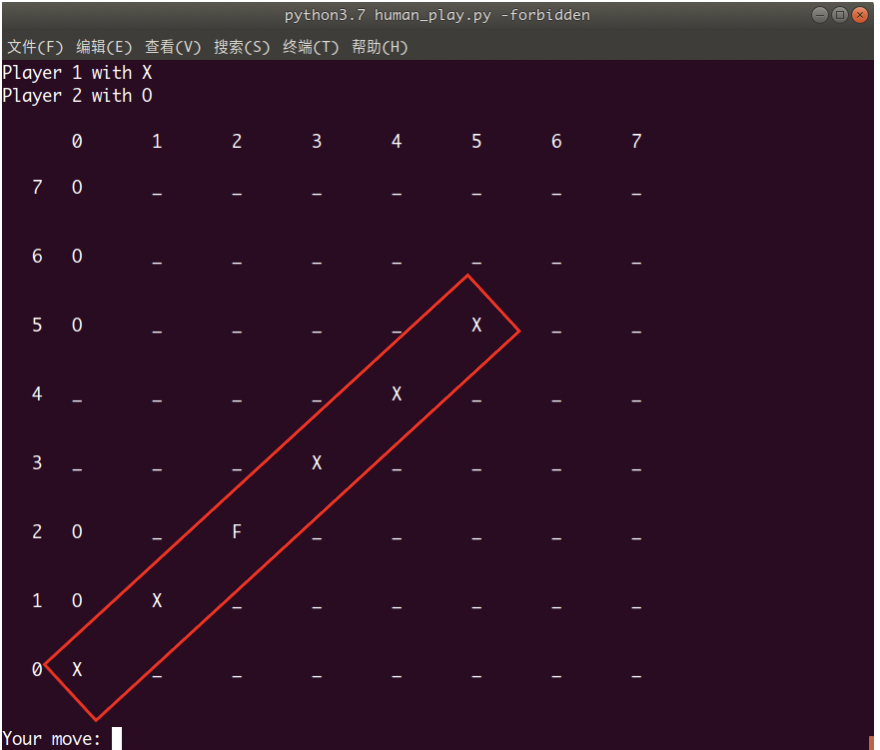
\includegraphics[width=0.85\linewidth]{./figs/l2.png}
                \end{minipage}%
                }%   
    
                \subfigure[long forbidden 3]{
                \begin{minipage}[t]{0.45\linewidth}
                \centering
                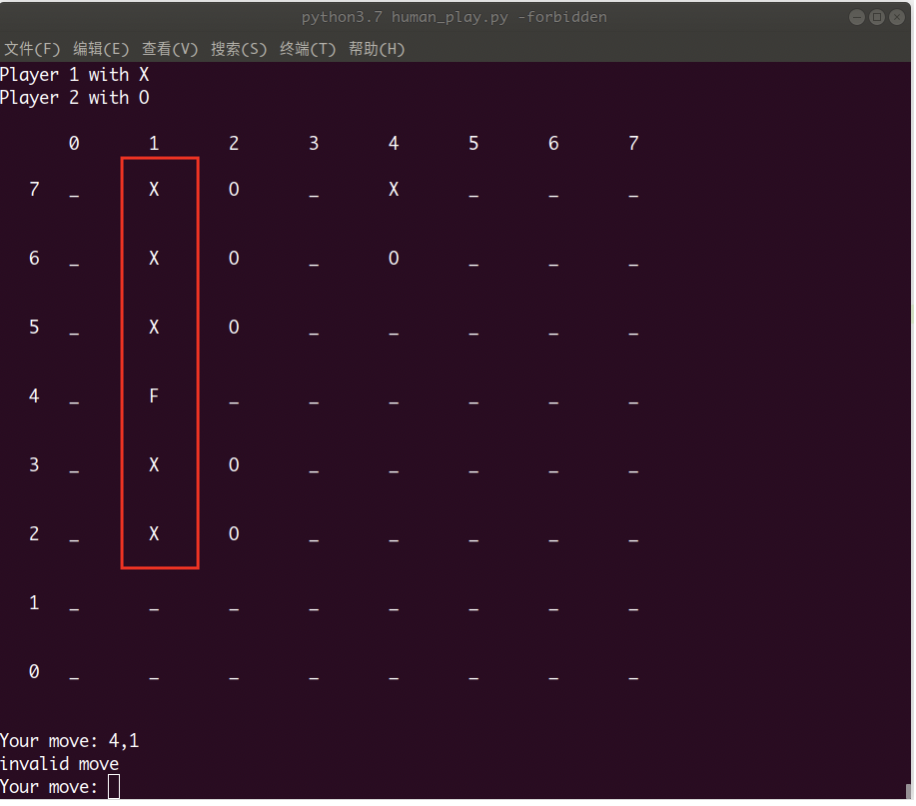
\includegraphics[width=0.85\linewidth]{./figs/l3.png}
                \end{minipage}%
                }%
                \subfigure[long forbidden 4]{
                \begin{minipage}[t]{0.45\linewidth}
                \centering
                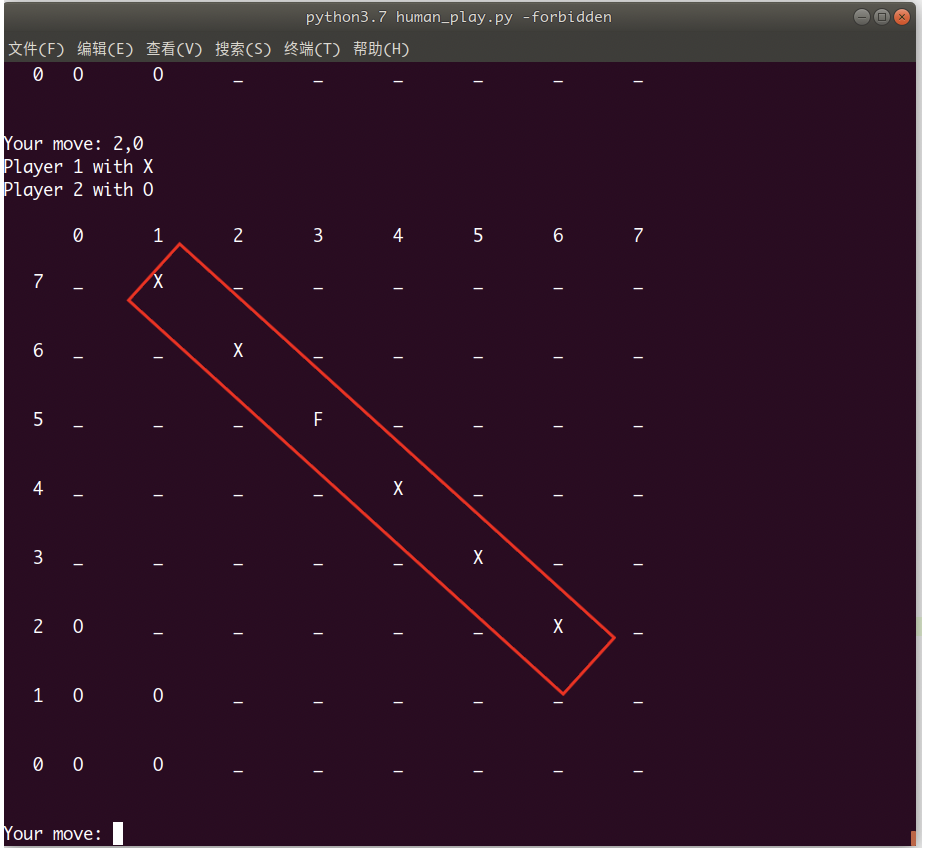
\includegraphics[width=0.85\linewidth]{./figs/l4.png}
                \end{minipage}%
                }%       
                \centering
            \end{figure}
            Then four-four forbidden rules (四四禁手 in Chinese) are implemented.\\
            First, consider the most simple cases:
            \begin{figure}[H]
                \centering
                \subfigure[44 forbidden-simple]{
                \begin{minipage}[t]{0.45\linewidth}
                \centering
                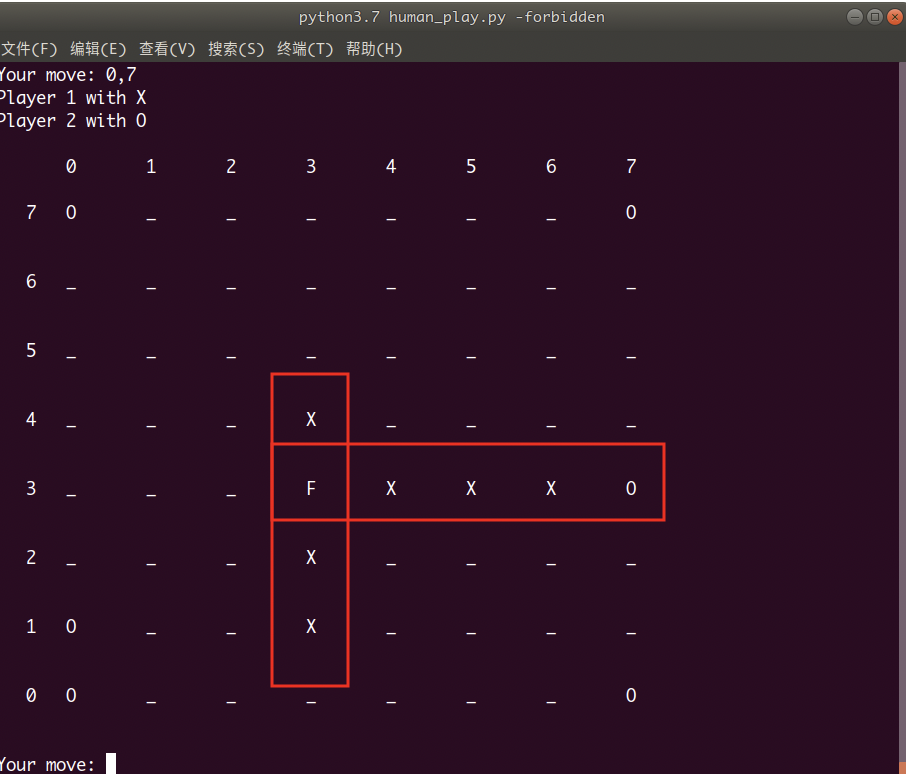
\includegraphics[width=0.85\linewidth]{./figs/440.png}
                \end{minipage}%
                }%
                \subfigure[44 forbidden-simple]{
                \begin{minipage}[t]{0.45\linewidth}
                \centering
                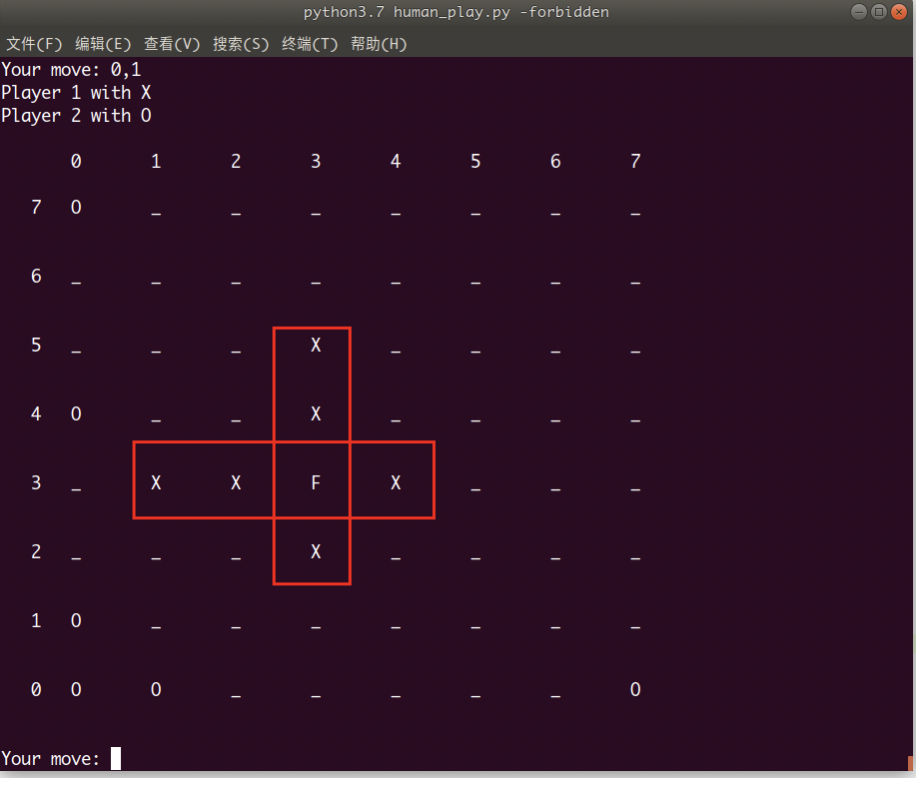
\includegraphics[width=0.85\linewidth]{./figs/441.png}
                \end{minipage}%
                }%   
            \end{figure}
            Let's check some special cases. The following 2 figures show that 
            if the chess are not continues, but need to be banned. The program 
            works quite well, it found the locations that need to be banned.
            \begin{figure}[H]
                \centering
                \subfigure[44 forbidden-case2]{
                \begin{minipage}[t]{0.45\linewidth}
                \centering
                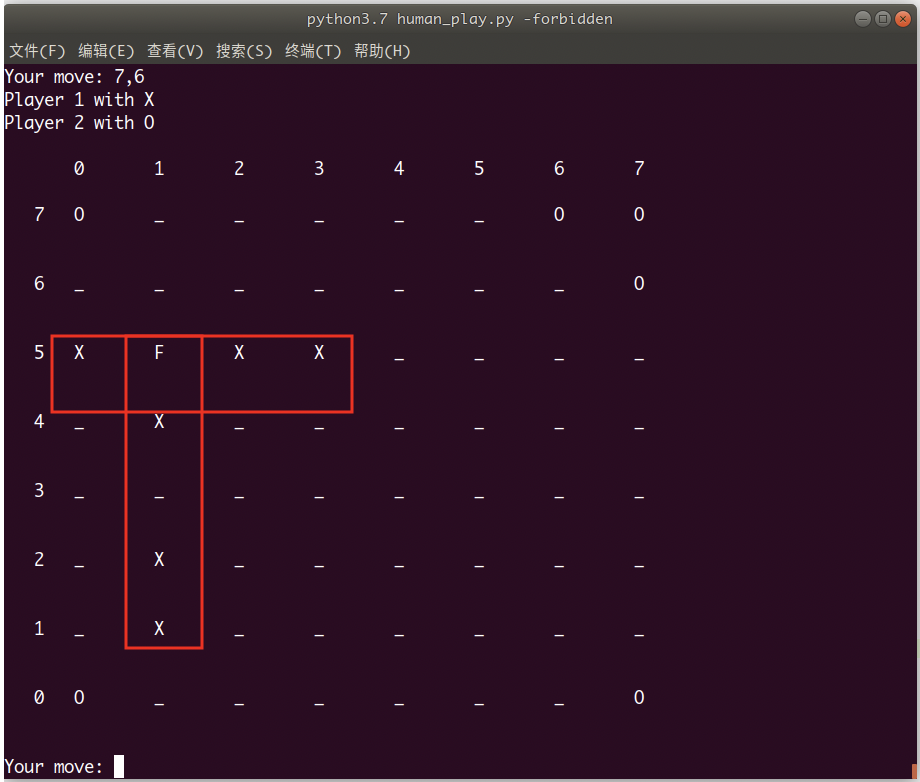
\includegraphics[width=0.85\linewidth]{./figs/442.png}
                \end{minipage}%
                }%
                \subfigure[44 forbidden-case2]{
                \begin{minipage}[t]{0.45\linewidth}
                \centering
                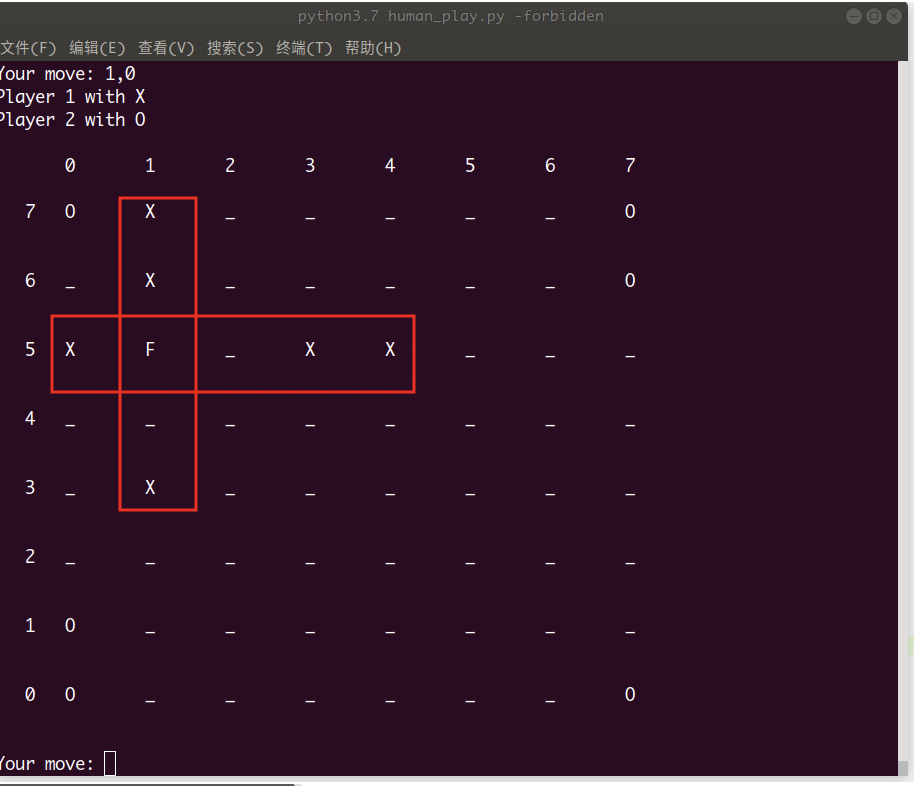
\includegraphics[width=0.85\linewidth]{./figs/443.png}
                \end{minipage}%
                }%   
            \end{figure}
            And it also works when there are multiple locations need to be banned:
            \begin{figure}[H]
                \centering
                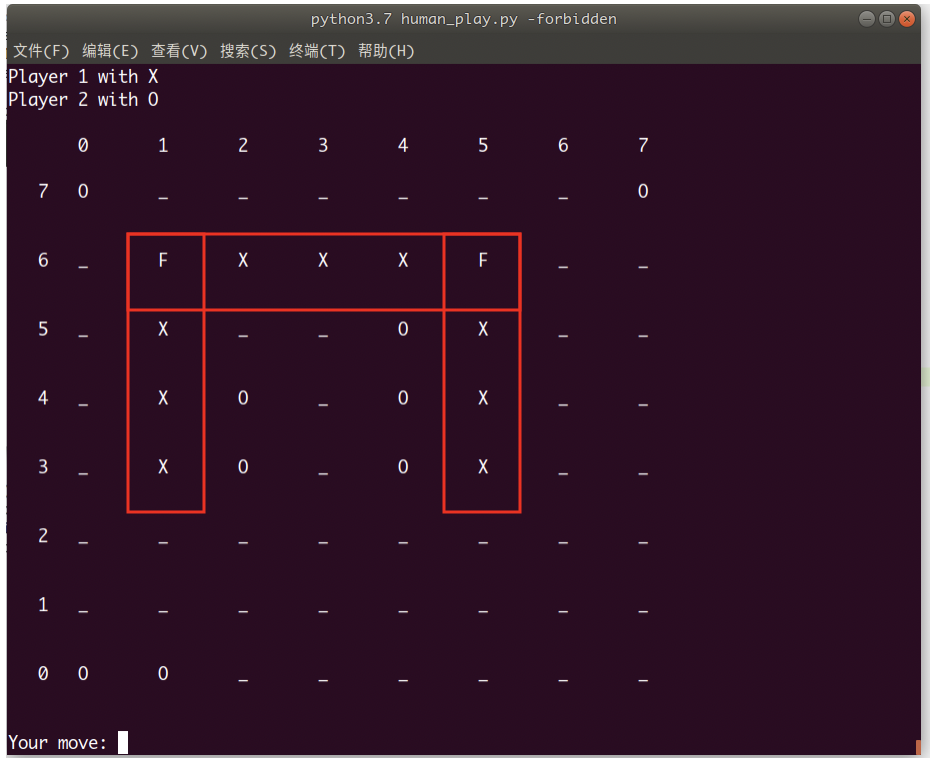
\includegraphics[scale=0.5]{./figs/444.png}
                \caption{44 forbidden-case3}
            \end{figure}
            And consider the following condition, the 4 chess in green rectangle is 
            not ``alive'' (不为活四或冲四, in Chinese). So there is only one ``alive'' 4-chess 
            chain here. 
            \begin{figure}[H]
                \centering
                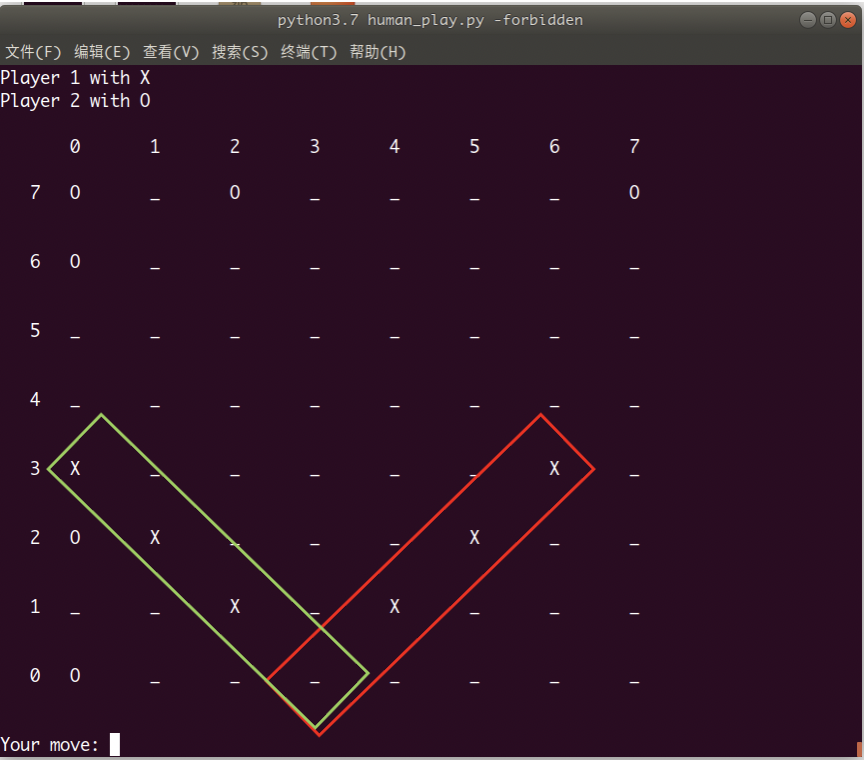
\includegraphics[scale=0.5]{./figs/44die.png}
                \caption{44 forbidden special}
            \end{figure}
            Then, consider the most special case. First we know, the 4 chess chain 
            in blue rectangle is not ``alive'', while that in yellow rectangle is alive. 
            What's more, if you put chess at $(3,3)$, you'll win the game directly. 
            In Chinese terms, it not satisfies ``有两个活四或冲四'', for you will win directly. Hence, 
            position $(3,3)$ can't be banned.
            \begin{figure}[H]
                \centering
                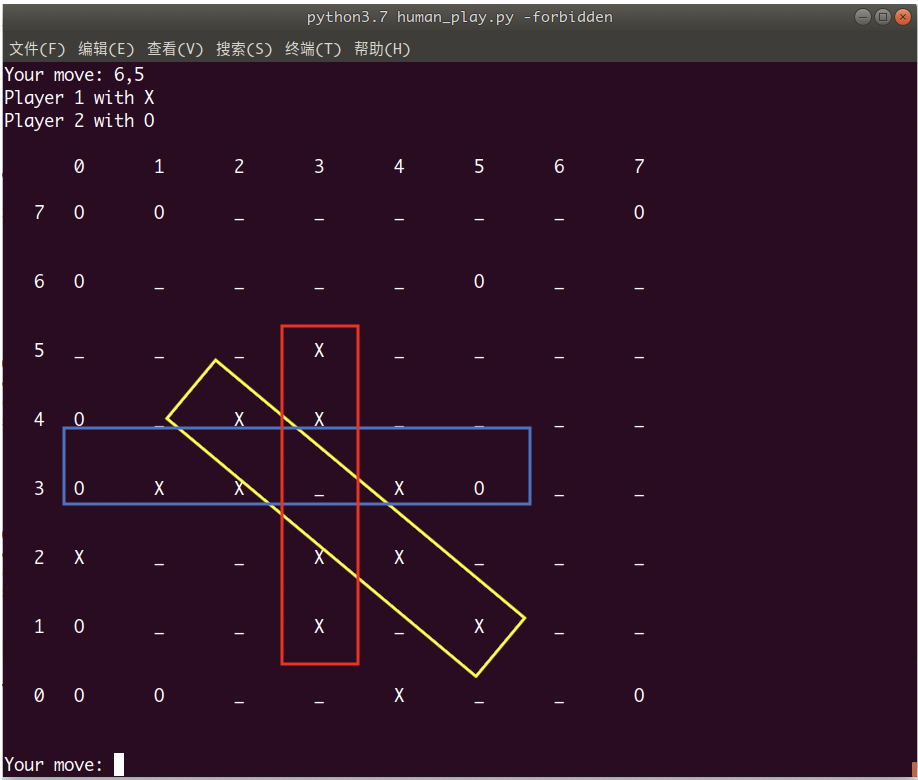
\includegraphics[scale=0.5]{./figs/44spec.png}
                \caption{44 forbidden special2}
            \end{figure}
            Finally, consider the 33 forbidden rules (三三禁手 in Chinese)
            We also start with the simplest conditions:
            \begin{figure}[H]
                \centering
                \subfigure[33 forbidden-simple]{
                \begin{minipage}[t]{0.45\linewidth}
                \centering
                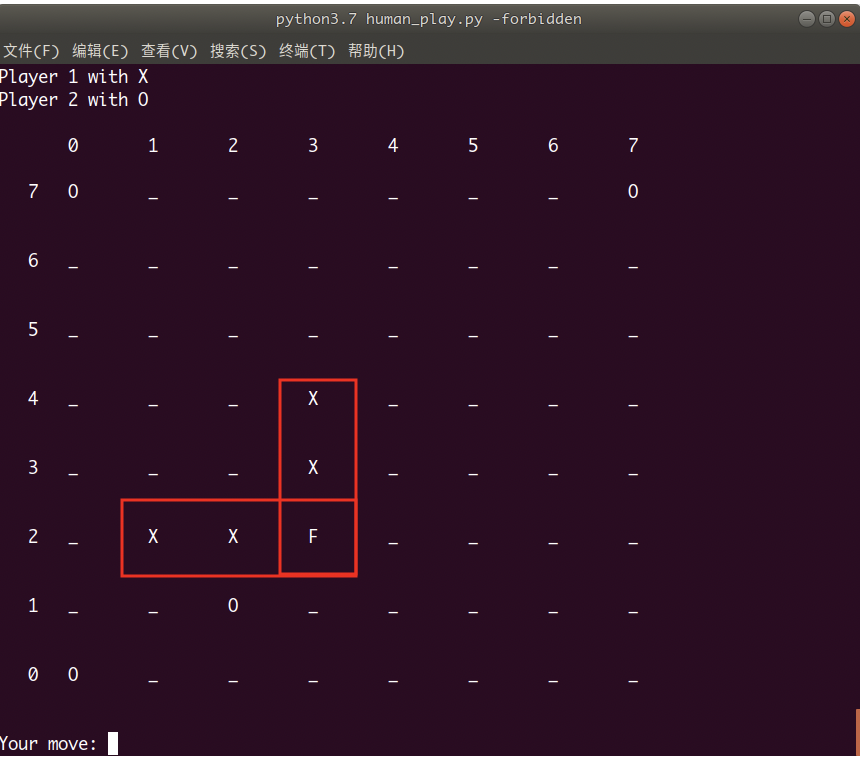
\includegraphics[width=0.85\linewidth]{./figs/330.png}
                \end{minipage}%
                }%
                \subfigure[33 forbidden-simple]{
                \begin{minipage}[t]{0.45\linewidth}
                \centering
                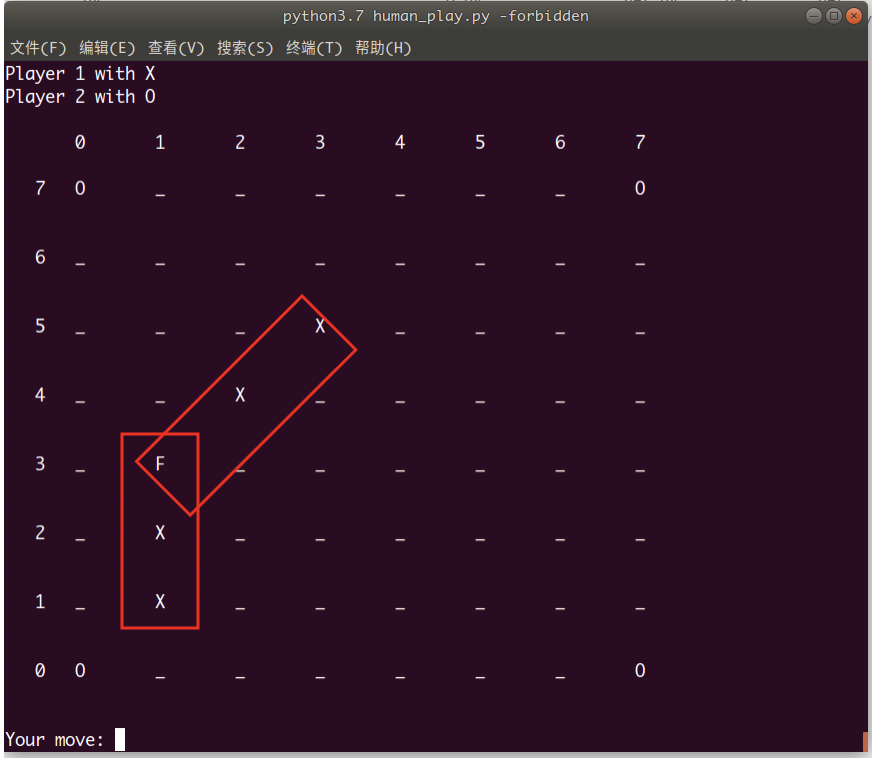
\includegraphics[width=0.85\linewidth]{./figs/331.png}
                \end{minipage}%
                }%   
            \end{figure}
            Then, some more complicated cases. First, the 33 chain which is not continues but 
            need to be banned.
            \begin{figure}[H]
                \centering
                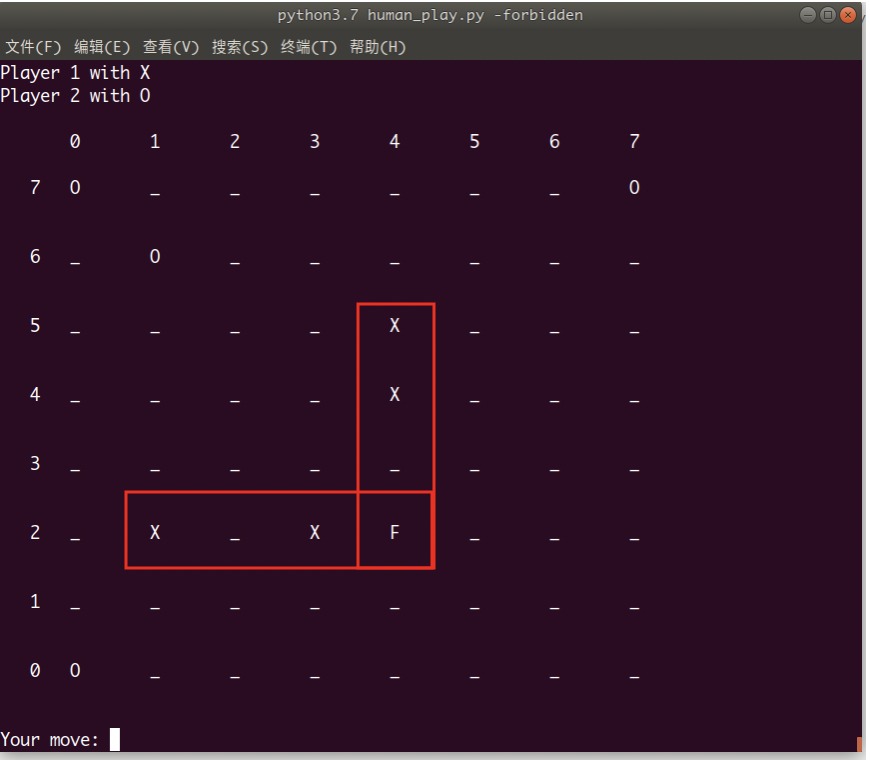
\includegraphics[scale=0.5]{./figs/332.png}
                \caption{33 forbidden-case2}
            \end{figure}
            It also works under multiple locations need to be banned:
            \begin{figure}[H]
                \centering
                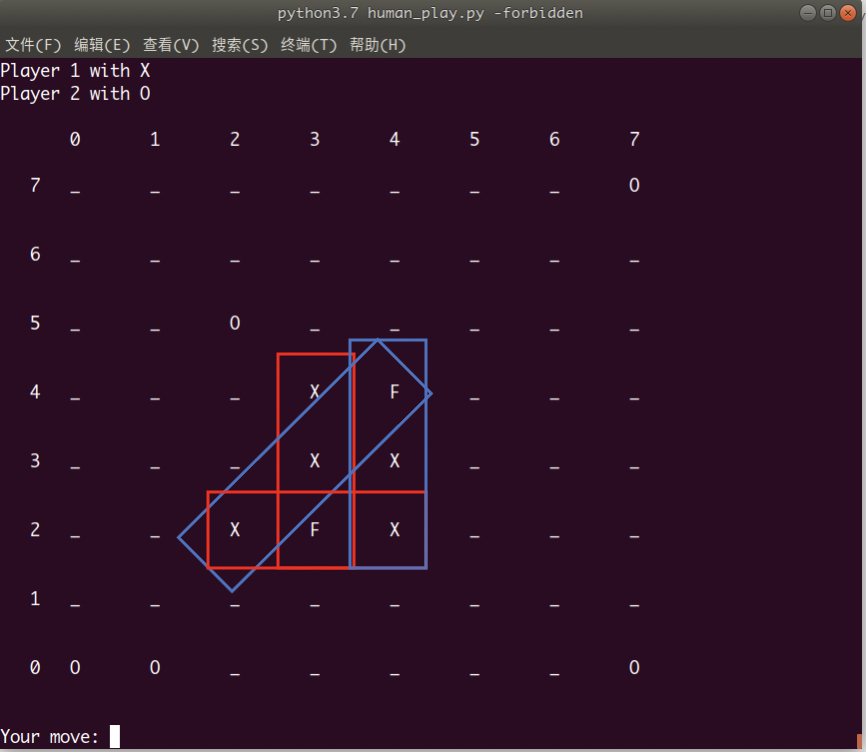
\includegraphics[scale=0.5]{./figs/334.png}
                \caption{33 forbidden multi-locations}
            \end{figure}
            \pagebreak
            Then, consider the following case. The chess in green rectangle is 
            named ``眠三'' in Chinese terms, which is not a ``alive'' 3-chess chain. So, postion $(2,4)$
            can't be banned.
            \begin{figure}[H]
                \centering
                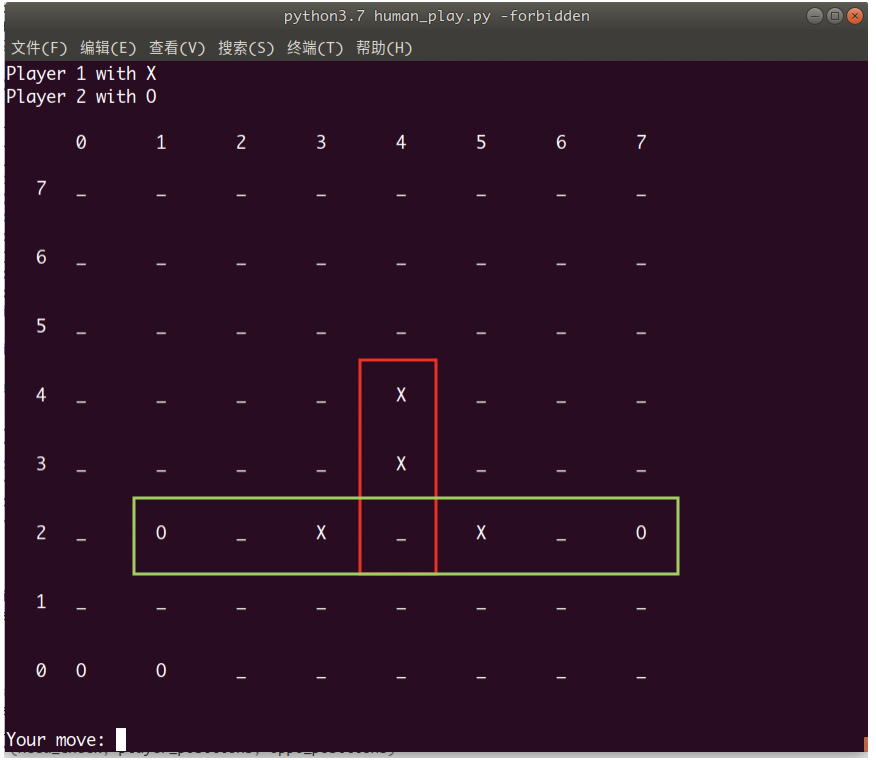
\includegraphics[scale=0.5]{./figs/333.png}
                \caption{33 forbidden-special}
            \end{figure}
        \item[2)] Gomoku RL agent with Forbidden Rule\\
            In this problem, I use the approximate Q-learning algorithm. \\
            The basic equation of this algorithm is:\\
            We use a linear expression to present a Q value $Q(s,a)$, assume there are $n$ parameters 
            are used:
            $$Q(s,a) = \sum_{i=1}^{n}w_i f_i(s,a)$$ 
            where $w_i$ are parameters that need to be learned, $f_i(s,a)$ are different feature functions to 
            evaluate the state-action pair $(s,a)$. \\
            Then, instead of updating $Q$ values in Bellman equation, we update the parameters $w_i$ instead. 
            By the original Bellman equation:
            $$Q(s,a) \gets Q(s,a) + \alpha (R_{s}^a + \gamma \max_{a'}Q(s',a') - Q(s,a))$$
            the Bellman equation in approximate Q learning is:
            $$w_i(s,a) \gets w_i(s,a) + \alpha (R_{s}^a + \gamma \max_{a'}Q(s',a') - Q(s,a))f_i(s,a)$$
            I consider following 4 features:
            \begin{enumerate}
                \item [1)] If there are agent's alive 3-chess chain after $(s,a)$. If there exist such 3 chess chain, 
                $f_1(s,a) = 1$, otherwise $f_1(s,a) = 0$
                \item [2)] If there are agent's alive 4-chess chain after $(s,a)$. If there exist such 4 chess chain, 
                $f_2(s,a) = 1$, otherwise $f_2(s,a) = 0$
                \item [3)] If there are opponent's alive 3-chess chain after $(s,a)$. If there exist such 3 chess chain, 
                $f_3(s,a) = 1$, otherwise $f_3(s,a) = 0$
                \item [4)] If there are opponent's alive 4-chess chain after $(s,a)$. If there exist such 4 chess chain, 
                $f_4(s,a) = 1$, otherwise $f_4(s,a) = 0$
            \end{enumerate}
            Then, the Q value can be represent as:
            $$Q(s,a) = w_1f_1(s,a) + w_2f_2(s,a) + w_3f_3(s,a) + w_4f_4(s,a)$$
            We know that, after taking action $a$, if there are agent's new 3 or 4 chess chain, 
            it's a good thing for the agent, it need to get some reward, so the weights of $f_1$ and $f_2$ should 
            be positive. But if there are opponent's chess chain, it's a bad thing for the agent, we need 
            to punish it with negative weights.\\
            Also, we need to balance the exploration and exploitation. I use $\epsilon$-greedy algorithm, 
            at first, $\epsilon=0.1$, and by the game tree going down, we need to decrease the $\epsilon$ to 
            make better decisions. Hence, I set 
            $$\epsilon = 0.1*\frac{\text{number of available moves}}{\text{number of total moves}}$$
            Some experiments are shown below (\textbf{WHITE} chess are agent's move):\\
            First, it knows ``How to win the game''. It's shown that it ``wants'' to make a 5-chess chain:
            \begin{figure}[H]
                \centering
                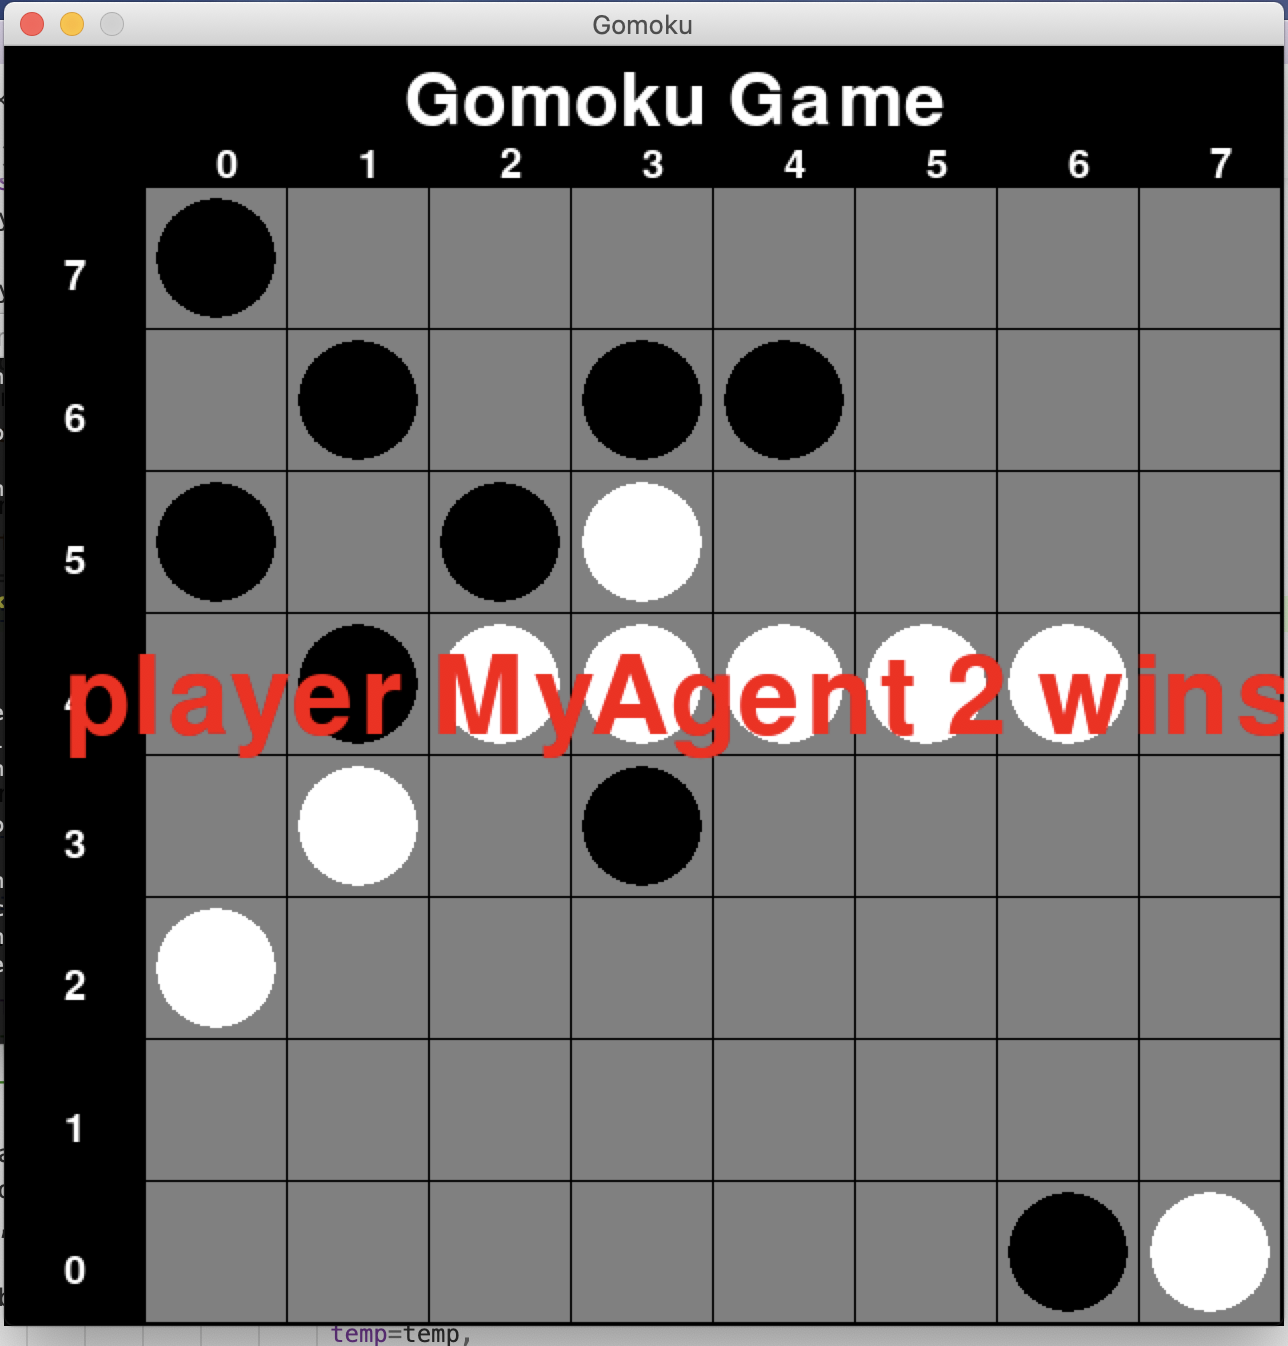
\includegraphics[scale=0.35]{./figs/win.png}
                \caption{It wins the game}
            \end{figure}
            Second, it knows to prevent its opponent from winning the game. It's shown that the agent
            puts chess on $(2,7)$ and $(2,2)$ to prevent me from winning the game.
            \begin{figure}[H]
                \centering
                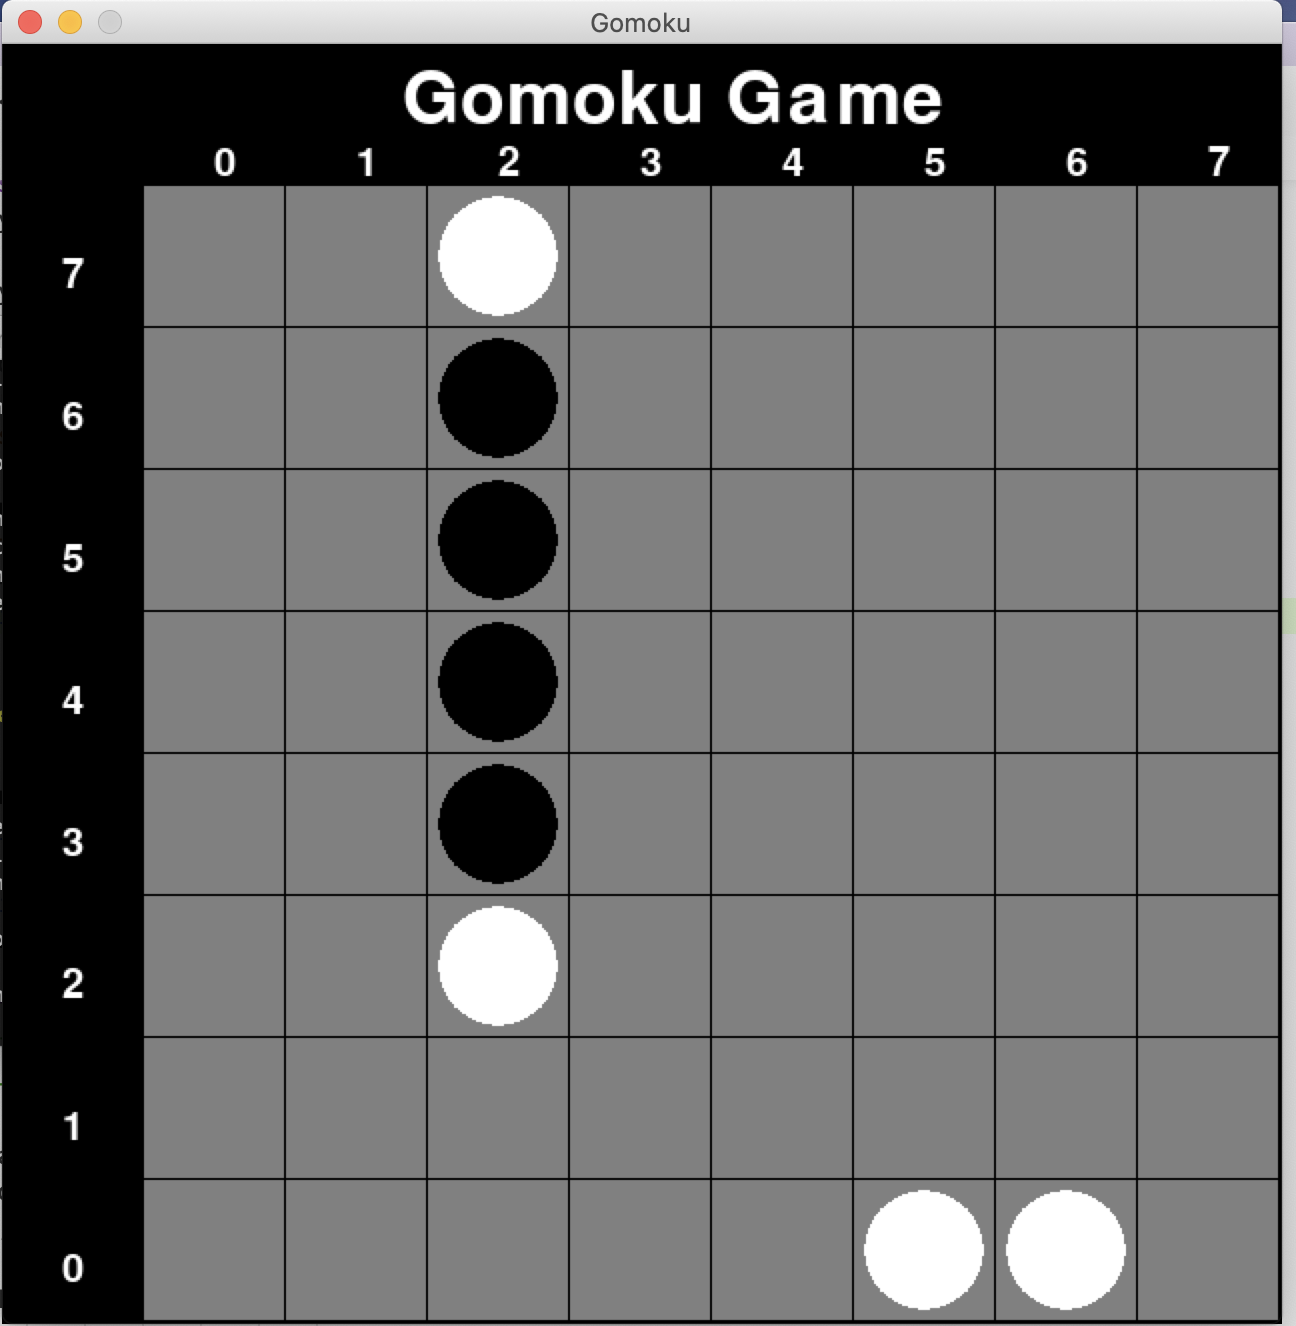
\includegraphics[scale=0.35]{./figs/prevent.png}
                \caption{It prevents me from winning}
            \end{figure}
            In experiments, it works well, when it play with \textbf{Pure MCTS 2000}, it wins 
            3 of 5 games, and 1 tie. But it still cannot win the AlphaZero with deep neural network (9 of 10 loses).
        \item[3)] Experiences
            \begin{enumerate}
                \item When implementing forbidden rules, it's really hard to 
                consider all the conditions. We need to traverse all empty positions, 
                then assume there is a black chess. Then use search based algorithm to 
                find if there are any positions need to be banned.
                \item Approximate Q learning works fine at this game. It's better and faster than 
                pure MCTS algorithm, and has shown relative high win rate while playing with MCTS. 
                For suitable feature functions are set, it can easily found some ``good'' locations.
                \item The disadvantage is, it needs human's prior knowledge. The feature functions 
                are selected by me manully, which is not very elegant. 
                \item It's important to balance the exploration and exploitation. At the beginning of the 
                game, we need to explore more, and by the game tree going down, we need to make it 
                choose to optimal policy with high probability.
            \end{enumerate}
        \item[4)] Innovative parts \\
            First, I make it much completed on the level of software engineering. 
            The command line argument parsing, usage, and error handling are all much 
            more completed, part of structure of the code is changed. (As shown in the Usage section)\\
            Second, I use a search and hypothesis based approach to find forbidden locations.  
            When implementing the forbidden rules, I use many testcases to 
            vaildate my implementation, and all of cases are passed. That means, 
            my implementation of forbidden rules almost included all possible conditions.
            Part of test results are shown in part(1). \\
            Then, I provided a GUI (shown in next page) that improved the interaction between AI and human.
            \begin{figure}[H]
                \centering
                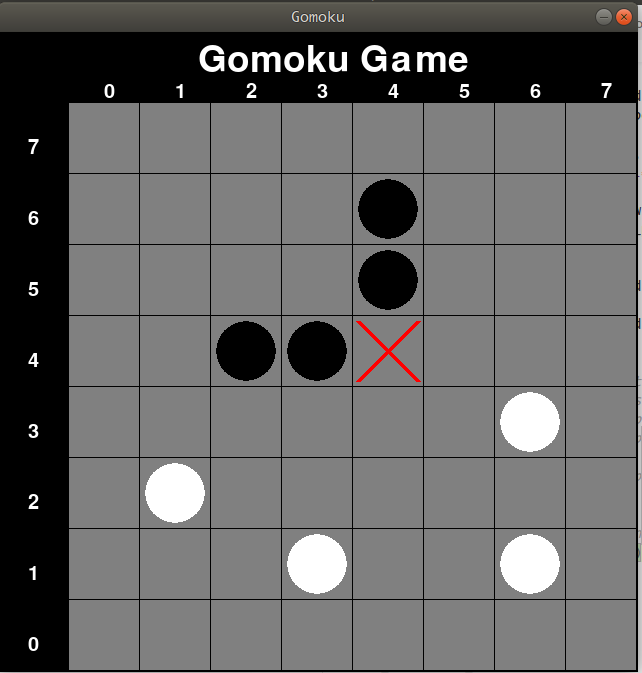
\includegraphics[scale=0.35]{./GUI.png}
                \caption{Pygame based GUI}
            \end{figure}
            You control the game using mouse instead of keyboard, which is much easier for human players.
        \end{enumerate}
\end{homeworkProblem}

\end{document}
